\documentclass{beamer}

\usetheme{Madrid}
\usecolortheme{default}

\usepackage{listings}
\usepackage{graphicx}
\usepackage{tikz}
\usepackage{booktabs}

\lstset{
  basicstyle=\ttfamily\scriptsize,
  breaklines=true,
  frame=single,
  backgroundcolor=\color{gray!10}
}

\title{AI-Assisted Operations}
\subtitle{Strategy and Tactics for AI usage in the jbox Project}
\author{Jordan Vieler}
\institute{UCSC Silicon Valley Extension \\ EMBD.X420 - Linux Systems Programming}
\date{December 17, 2025}

\begin{document}

% -----------------------------------------------------------------------------
% Title
% -----------------------------------------------------------------------------
\begin{frame}
  \titlepage
\end{frame}

% -----------------------------------------------------------------------------
% Table of Contents
% -----------------------------------------------------------------------------
\begin{frame}
  \frametitle{Outline}
  \scriptsize
  \setbeamertemplate{section in toc}{\textbullet~\inserttocsection\par}
  \linespread{0.8}\selectfont
  \vspace{-0.5em}
  \tableofcontents[hideallsubsections]
\end{frame}

% =============================================================================
% SECTION: Overview
% =============================================================================
\section{Development Cycle}

\begin{frame}{Development Cycle}
  The development process follows a \textbf{plan-implement-verify-commit} cycle
  that maximizes AI effectiveness while maintaining code quality.

  \vspace{1em}
  \begin{center}
  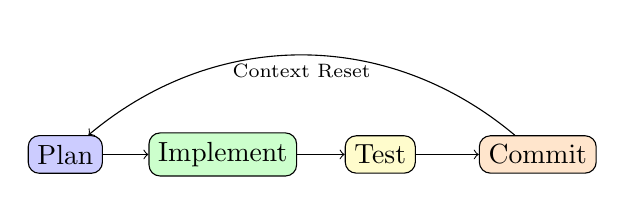
\begin{tikzpicture}[node distance=2cm, auto]
    \node[draw, rounded corners, fill=blue!20] (plan) {Plan};
    \node[draw, rounded corners, fill=green!20, right of=plan] (impl) {Implement};
    \node[draw, rounded corners, fill=yellow!20, right of=impl] (test) {Test};
    \node[draw, rounded corners, fill=orange!20, right of=test] (commit) {Commit};

    \draw[->] (plan) -- (impl);
    \draw[->] (impl) -- (test);
    \draw[->] (test) -- (commit);
    \draw[->, bend right=40] (commit) to node[below] {\scriptsize Context Reset} (plan);
  \end{tikzpicture}
  \end{center}

  \vspace{1em}
  Key principle: \textbf{Incremental progress with context resets} maintains
  coherence across sessions.
\end{frame}

% =============================================================================
% SECTION: Branching Strategy
% =============================================================================
\section{Branching Strategy}

\begin{frame}{Branching Strategy}{Workflow}
  AI-assisted development uses a dedicated branch to isolate AI work:

  \vspace{0.5em}
  \begin{enumerate}
    \item \textbf{Create AI branch} --- Branch off from current dev/feature branch
    \item \textbf{AI performs work} --- All implementation on the \texttt{ai} branch
    \item \textbf{Merge to dev/feature} --- Once complete, merge back
    \item \textbf{Merge to master} --- Final integration
  \end{enumerate}

  \vspace{1em}
  \begin{center}
  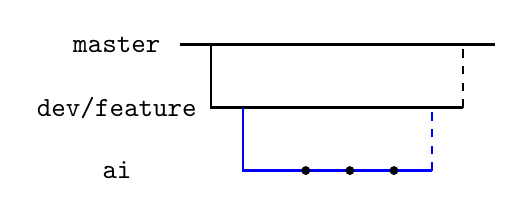
\begin{tikzpicture}[scale=0.8]
    \node at (0, 2) {\texttt{master}};
    \draw[thick] (1, 2) -- (6, 2);

    \node at (0, 1) {\texttt{dev/feature}};
    \draw[thick] (1.5, 2) -- (1.5, 1) -- (5.5, 1);
    \draw[thick, dashed] (5.5, 1) -- (5.5, 2);

    \node at (0, 0) {\texttt{ai}};
    \draw[thick, blue] (2, 1) -- (2, 0) -- (5, 0);
    \draw[thick, blue, dashed] (5, 0) -- (5, 1);

    \fill (3, 0) circle (2pt);
    \fill (3.7, 0) circle (2pt);
    \fill (4.4, 0) circle (2pt);
  \end{tikzpicture}
  \end{center}
\end{frame}

\begin{frame}{Branching Strategy}{Benefits}
  \begin{itemize}
    \item \textbf{Isolation} --- AI work is separated from ongoing development
    \vspace{0.5em}
    \item \textbf{Review opportunity} --- Changes can be reviewed before merging
    \vspace{0.5em}
    \item \textbf{Easy rollback} --- Branch can be discarded if issues arise
    \vspace{0.5em}
    \item \textbf{Clean history} --- Squash merges consolidate AI commits
  \end{itemize}
\end{frame}

% =============================================================================
% SECTION: Project Setup
% =============================================================================
\section{Project Setup}

\begin{frame}{Project Setup}{Establish Conventions Early}
  Before implementation, establish clear conventions the AI will follow:

  \vspace{1em}
  \begin{description}
    \item[\texttt{CONVENTIONS.md}] Code style, naming, standards (C23, etc.)
    \item[\texttt{APPANATOMY.md}] Standard command structure and modules
    \item[\texttt{CLItools.md}] CLI specification for agent-facing commands
    \item[\texttt{CLAUDE.md}] Project-level instructions for the AI
  \end{description}

  \vspace{1em}
  \textbf{Key insight:} Specification files define \emph{target architecture}
  before features are implemented, ensuring coherence across the codebase.
\end{frame}

\begin{frame}{Project Setup}{Standardize Testing}
  Choose a single testing framework and format:

  \vspace{1em}
  \begin{itemize}
    \item \textbf{Python unittest} for all tests in this project
    \vspace{0.5em}
    \item Consistent naming: \texttt{test\_<component>.py}
    \vspace{0.5em}
    \item Consistent structure: \texttt{tests/<category>/<component>/}
    \vspace{0.5em}
    \item Tests generated \emph{alongside} implementation
  \end{itemize}

  \vspace{1em}
  \begin{block}{Benefit}
    Uniform testing structure allows AI to generate tests consistently
    without needing repeated instructions.
  \end{block}
\end{frame}

% =============================================================================
% SECTION: Feature Implementation Workflow
% =============================================================================
\section{Feature Implementation Workflow}

\begin{frame}{Feature Implementation}{Phase 1: Planning}
  \textbf{Write a Detailed Specification:}
  \begin{itemize}
    \item Feature requirements and behavior
    \item Input/output specifications
    \item Edge cases and error handling
    \item Integration points with existing code
  \end{itemize}

  \vspace{1em}
  \textbf{Generate Implementation Plan:}
  \begin{itemize}
    \item Ask AI to output \texttt{AI\_TODO\_<N>.md}
    \item Include phase breakdown with milestones
    \item Task checklists with \texttt{[ ]} checkboxes
    \item File locations and dependencies
  \end{itemize}
\end{frame}

\begin{frame}[fragile]{Feature Implementation}{Phase 2: Implementation}
  Instruct the AI to execute with clear constraints:

  \vspace{0.5em}
  \begin{lstlisting}
Proceed with the implementation plan in AI_TODO_<N>.md.

Constraints:
- Check off todos as they are completed
- Generate tests in the appropriate directory
- Update Makefile targets when necessary
- Follow conventions in CONVENTIONS.md
- Generate Doxygen-style docstrings
- Commit changes after each implementation phase
  \end{lstlisting}

  \vspace{0.5em}
  \textbf{Incremental Progress:}
  Implement $\rightarrow$ Test $\rightarrow$ Update build $\rightarrow$
  Mark complete $\rightarrow$ Commit
\end{frame}

\begin{frame}{Feature Implementation}{Phase 3: Context Management}
  After each major phase or commit:

  \vspace{1em}
  \begin{enumerate}
    \item \textbf{Reset the conversation context} (start fresh session)
    \item Instruct AI to continue from where it left off
    \item Reference the \texttt{AI\_TODO\_<N>.md} file as persistent state
  \end{enumerate}

  \vspace{1em}
  \begin{alertblock}{Why Reset Context?}
    \begin{itemize}
      \item Prevents context overflow in long implementations
      \item Maintains fresh, focused sessions
      \item \texttt{AI\_TODO} file serves as the ``memory''
    \end{itemize}
  \end{alertblock}
\end{frame}

% =============================================================================
% SECTION: Quick Changes Workflow
% =============================================================================
\section{Quick Changes Workflow}

\begin{frame}{Quick Changes Workflow}
  For small changes that don't require extensive planning:

  \vspace{1em}
  \begin{center}
    \textbf{Change} $\longrightarrow$ \textbf{Test} $\longrightarrow$ \textbf{Commit}
  \end{center}

  \vspace{1em}
  \textbf{Characteristics:}
  \begin{itemize}
    \item Single session, no plan required
    \item Changes made directly
    \item Tests run to verify
    \item Committed immediately
  \end{itemize}

  \vspace{1em}
  \textbf{Examples:}
  Bug fixes, documentation updates, small refactors, configuration changes
\end{frame}

% =============================================================================
% SECTION: Debugging Workflow
% =============================================================================
\section{Debugging Workflow}

\begin{frame}[fragile]{Debugging Workflow}
  When tests fail or bugs are detected:

  \vspace{0.5em}
  \begin{enumerate}
    \item \textbf{Reset context} if necessary (avoid confusion)
    \item \textbf{Provide clear bug report:}
  \end{enumerate}

  \begin{lstlisting}
A bug has been detected in <component>.

Symptoms:
- <what is happening>

Expected behavior:
- <what should happen>

Relevant files:
- <file paths>

Test output:
<paste failing test output>
  \end{lstlisting}

  \vspace{0.5em}
  AI then: Analyze $\rightarrow$ Identify root cause $\rightarrow$
  Fix $\rightarrow$ Verify $\rightarrow$ Commit
\end{frame}

% =============================================================================
% SECTION: Documentation Standards
% =============================================================================
\section{Documentation Standards}

\begin{frame}[fragile]{Documentation Standards}{Doxygen-Style Docstrings}
  All functions include documentation:

  \vspace{0.5em}
  \begin{lstlisting}[language=C]
/**
 * @brief Short description of the function
 *
 * Longer description if needed, explaining
 * behavior, edge cases, and important details.
 *
 * @param param1 Description of first parameter
 * @param param2 Description of second parameter
 * @return Description of return value
 */
int function_name(int param1, char *param2);
  \end{lstlisting}
\end{frame}

\begin{frame}[fragile]{Documentation Standards}{AI\_TODO File Format}
  Implementation plans follow a consistent structure:

  \begin{lstlisting}
# Feature Implementation Plan

## Overview
Brief description of what's being implemented.

## Phase 1: Component Name
### 1.1 Task Group
- [ ] Specific task
- [ ] Another task

## Phase 2: Next Component
...

## Notes
Additional context, dependencies, considerations.
  \end{lstlisting}
\end{frame}

% =============================================================================
% SECTION: Best Practices
% =============================================================================
\section{Best Practices}

\begin{frame}{Best Practices}{Do}
  \begin{itemize}
    \item \textbf{Be specific} in requirements and constraints
    \vspace{0.5em}
    \item \textbf{Break large features} into multiple phases
    \vspace{0.5em}
    \item \textbf{Reset context} between major phases
    \vspace{0.5em}
    \item \textbf{Verify plans} before implementation
    \vspace{0.5em}
    \item \textbf{Test incrementally} as features are built
    \vspace{0.5em}
    \item \textbf{Commit frequently} with descriptive messages
  \end{itemize}
\end{frame}

\begin{frame}{Best Practices}{Don't}
  \begin{itemize}
    \item Don't let context grow too large
    \vspace{0.5em}
    \item Don't skip the planning phase for complex features
    \vspace{0.5em}
    \item Don't implement without tests
    \vspace{0.5em}
    \item Don't ignore failing tests
    \vspace{0.5em}
    \item Don't forget to update build system
  \end{itemize}
\end{frame}

% =============================================================================
% SECTION: Session Templates
% =============================================================================
\section{Session Templates}

\begin{frame}[fragile]{Session Templates}{New Feature Session}
  \begin{lstlisting}
Implement <feature> for the jbox project.

<detailed requirements>

Output an implementation plan as AI_TODO_<N>.md
following the format in existing AI_TODO files.
  \end{lstlisting}
\end{frame}

\begin{frame}[fragile]{Session Templates}{Continue Implementation Session}
  \begin{lstlisting}
Continue with the implementation plan in
ai/plans/AI_TODO_<N>.md.

Resume from Phase <X>.

Constraints:
- Check off todos as completed
- Generate tests in tests/<category>/
- Update Makefile when needed
- Use Doxygen-style docstrings
- Follow CONVENTIONS.md
- Commit after each phase
  \end{lstlisting}
\end{frame}

\begin{frame}[fragile]{Session Templates}{Bug Fix \& Quick Change}
  \textbf{Bug Fix:}
  \begin{lstlisting}
Debug the following issue in <component>:

<bug description and test output>

Fix the bug and verify with tests.
  \end{lstlisting}

  \vspace{1em}
  \textbf{Quick Change:}
  \begin{lstlisting}
<describe the change needed>

Make the change, test it, and commit.
  \end{lstlisting}
\end{frame}

% =============================================================================
% SECTION: Summary
% =============================================================================
\section{Workflow Summary}

\begin{frame}{Workflow Summary}
  \begin{table}
    \centering
    \begin{tabular}{ll}
      \toprule
      \textbf{Scenario} & \textbf{Approach} \\
      \midrule
      New major feature & Plan $\rightarrow$ Implement $\rightarrow$ Test
                          $\rightarrow$ Commit $\rightarrow$ Reset \\
      Small change & Change $\rightarrow$ Test $\rightarrow$ Commit \\
      Bug fix & Reset $\rightarrow$ Debug $\rightarrow$ Fix
                $\rightarrow$ Test $\rightarrow$ Commit \\
      Documentation & Write $\rightarrow$ Review $\rightarrow$ Commit \\
      \bottomrule
    \end{tabular}
  \end{table}

  \vspace{1em}
  This strategy enables efficient AI-assisted development while maintaining
  \textbf{code quality}, \textbf{consistency}, and \textbf{project coherence}.
\end{frame}

% =============================================================================
% SECTION: Key Takeaways
% =============================================================================
\section{Key Takeaways}

\begin{frame}{Key Takeaways}{Lessons Learned}
  \begin{enumerate}
    \item \textbf{AI works best on well-defined incremental changes}
    \begin{itemize}
      \item Small, focused tasks yield better results than large ambiguous ones
    \end{itemize}

    \vspace{0.5em}
    \item \textbf{Project structure matters}
    \begin{itemize}
      \item Modular design allows changes to slot in cleanly
      \item Tests can be added systematically
      \item Build system can be easily expanded
    \end{itemize}

    \vspace{0.5em}
    \item \textbf{Simple, statically-typed languages help}
    \begin{itemize}
      \item C with well-established best practices
      \item AI translates specifications to code more consistently
      \item Clear contracts reduce ambiguity
    \end{itemize}
  \end{enumerate}
\end{frame}

\begin{frame}{Key Takeaways}{Lessons Learned (cont.)}
  \begin{enumerate}
    \setcounter{enumi}{3}
    \item \textbf{AI struggles with contract changes}
    \begin{itemize}
      \item Updating callers when interfaces change is error-prone
      \item Since ``generating'' code is cheap, define first:
      \begin{enumerate}
        \item Architecture and contracts
        \item Dependencies
        \item Tests
      \end{enumerate}
      \item Then generate tests, then proceed with implementation
    \end{itemize}

    \vspace{1em}
    \item \textbf{Design before generation}
    \begin{itemize}
      \item Front-load architectural decisions
      \item Use specification documents as the source of truth
      \item Let AI implement against a predetermined design
    \end{itemize}
  \end{enumerate}
\end{frame}

\begin{frame}{Key Takeaways}{The Formula}
  \begin{center}
    \Large
    \textbf{Well-Defined Structure} \\
    + \\
    \textbf{Clear Specifications} \\
    + \\
    \textbf{Incremental Changes} \\
    = \\
    \textbf{Effective AI-Assisted Development}
  \end{center}
\end{frame}

% -----------------------------------------------------------------------------
% End
% -----------------------------------------------------------------------------
\begin{frame}
  \begin{center}
    \Huge Questions?
  \end{center}
\end{frame}

\end{document}
